% Titre de la premiere partie
\section{\fstpti}

%%%%%%%%%%%%%%%%%%%%%%%%%%%%%%%%%%%%%%%%%%%%%%%%
% Première diapo
%%%%%%%%%%%%%%%%%%%%%%%%%%%%%%%%%%%%%%%%%%%%%%%%
\begin{frame}
\frametitle{\fstpti}
\framesubtitle{Deux points de vue}

\begin{figure}
	\centering
	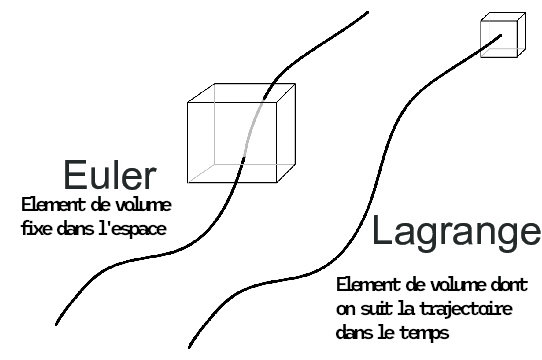
\includegraphics[width=0.8\linewidth]{figures/eulerian_vs_lagrangian_description.png}
\end{figure}

\end{frame}


%%%%%%%%%%%%%%%%%%%%%%%%%%%%%%%%%%%%%%%%%%%%%%%%
% Deuxième diapo
%%%%%%%%%%%%%%%%%%%%%%%%%%%%%%%%%%%%%%%%%%%%%%%%
\begin{frame}
\frametitle{\fstpti}
\framesubtitle{La description Eulerienne}

\noindent
\begin{minipage}[t]{0.6\textwidth}
	Caractéristiques:
	\begin{itemize}
		\item Élément de volume fixe dans l'espace
		\item Les variables d'intéret sont de la forme: $A(M,t)$
	\end{itemize}
\end{minipage}%
\begin{minipage}[t]{0.4\textwidth}
	\adjustimage{width=1.0\textwidth,valign=t}{figures/eulerian_representation.png}
\end{minipage}


\end{frame}


%%%%%%%%%%%%%%%%%%%%%%%%%%%%%%%%%%%%%%%%%%%%%%%%
% Troisième diapo
%%%%%%%%%%%%%%%%%%%%%%%%%%%%%%%%%%%%%%%%%%%%%%%%
\begin{frame}
\frametitle{\fstpti}
\framesubtitle{La description Lagrangienne}

\noindent
\begin{minipage}[t]{0.6\textwidth}
	Caractéristiques:
	\begin{itemize}
		\item Élément de volume bouge dans l'espace
		\item Les variables d'intéret sont de la forme: $A(M_0,t)$
	\end{itemize}
\end{minipage}%
\begin{minipage}[t]{0.4\textwidth}
	\adjustimage{width=1.0\textwidth,valign=t}{figures/lagrangian_representation.png}
\end{minipage}

\end{frame}


%%%%%%%%%%%%%%%%%%%%%%%%%%%%%%%%%%%%%%%%%%%%%%%%
% Quatrième diapo
%%%%%%%%%%%%%%%%%%%%%%%%%%%%%%%%%%%%%%%%%%%%%%%%
\begin{frame}
	\frametitle{\fstpti}
	\framesubtitle{Choix pour mon projet}

	\noindent
	\begin{minipage}[t]{0.5\textwidth}
		Eulerienne:
		\begin{itemize}
			\item Préférée pour la résolution des équations de Navier-Stokes
			\item Préférée pour modélisation de grands systèmes fluides
		\end{itemize}

	\end{minipage}%
	\begin{minipage}[t]{0.5\textwidth}
		Lagrangienne:
		\begin{itemize}
			\item Utile pour des problèmes où les trajectoires des particules sont cruciales
			\item Par exemple la simulation des mouvements de particules de fluide
		\end{itemize}

	\end{minipage}
	\newline
	\newline
	\newline
	\begin{minipage}[b]{0.5\textwidth}
		\textcolor{red}{\xmark} Utilisation non pertinente
	\end{minipage}%	
	\begin{minipage}[b]{0.5\textwidth}
		\textcolor{green}{\cmark} Utilisation pertinente
	\end{minipage}%


\end{frame}

%%%%%%%%%%%%%%%%%%%%%%%%%%%%%%%%%%%%%%%%%%%%%%%%
% Cinquieme diapo
%%%%%%%%%%%%%%%%%%%%%%%%%%%%%%%%%%%%%%%%%%%%%%%%
\begin{frame}
	\frametitle{\fstpti}
	\framesubtitle{Les équations du mouvement d'une particule de fluide}

	Pour une particule de fluide de volume $d\tau$ de masse $m$ et de masse volumique $\rho$, la 2nde loi de newton s'écrit:
	\begin{align*}
	m \frac{d\vec{v}}{dt} &= \vec{F}_{contact} + \vec{F}_{distance}
	\end{align*}

\end{frame}

%%%%%%%%%%%%%%%%%%%%%%%%%%%%%%%%%%%%%%%%%%%%%%%%
% Sixieme diapo
%%%%%%%%%%%%%%%%%%%%%%%%%%%%%%%%%%%%%%%%%%%%%%%%
\begin{frame}
	\frametitle{\fstpti}
	\framesubtitle{Les forces à distance}
	Forces à distances:
	\begin{itemize}
		\item Le poids: $\vec{P} = m \vec{g} = \rho d\tau \vec{g}$ 
		\item La force de Lorentz: $\vec{F_L} = q(\vec{E} + \vec{v}\wedge \vec{B}) = \vec{0}$
	\end{itemize}
	
	\hfill

	
	Expression:
	\begin{align*}
		\Aboxed{\vec{F}_{distance} = \rho d\tau \vec{g}}
	\end{align*}

\end{frame}

%%%%%%%%%%%%%%%%%%%%%%%%%%%%%%%%%%%%%%%%%%%%%%%%
% Septieme diapo
%%%%%%%%%%%%%%%%%%%%%%%%%%%%%%%%%%%%%%%%%%%%%%%%
\begin{frame}
	\frametitle{\fstpti}
	\framesubtitle{Les forces de contact}

	\noindent
	\begin{minipage}[t]{0.6\textwidth}
		Décomposition de la force de contact
		\begin{align*}
			d\vec{F}_{contact} = \underbrace{d\vec{F}_{tangentielle}}_\text{Viscosite} 	+ \underbrace{d\vec{F}_{normale}}_\text{Pression}
		\end{align*}
	\end{minipage}%
	\begin{minipage}[t]{0.4\textwidth}
		\adjustimage{width=1.0\textwidth,valign=t}{figures/force_de_contact_particule_de_fluide.png}
	\end{minipage}

	Après calculs on obtient les expressions suivantes:

	\noindent
	\begin{minipage}[t]{0.5\textwidth}
		\begin{align*}
			\Aboxed{d\vec{F}_{pression} = -\vec{\text{grad}}(P)d\tau}
		\end{align*}
	\end{minipage}%
	\begin{minipage}[t]{0.5\textwidth}
		\begin{align*}
			\Aboxed{d\vec{F}_{viscosite} = \eta \Delta \vec{v} d\tau}
		\end{align*}
	\end{minipage}

\end{frame}

%%%%%%%%%%%%%%%%%%%%%%%%%%%%%%%%%%%%%%%%%%%%%%%%
% Huitième diapo
%%%%%%%%%%%%%%%%%%%%%%%%%%%%%%%%%%%%%%%%%%%%%%%%

\begin{frame}
	\frametitle{\fstpti}
	\framesubtitle{Les équations de Navier-Stokes}
	
	Équation de conservation de la quantité de mouvement:
	\begin{align*}
		\Aboxed{\rho \Big [\frac{\partial \vec{v}}{\partial t} +\vec{v} \cdot \vec{\text{grad}}(v) \Big ]= \rho \vec{g} - \vec{grad} P + \eta \Delta \vec{v} + \vec{F}}
	\end{align*}

	Équation de conservation de la masse:
	\begin{align*}
		\Aboxed{\frac{\partial \rho}{\partial t} + \rho \text{div } \vec{v} = 0}
	\end{align*}

\end{frame}
